\chapter{Cognitive explorations}
\label{sec:5}
\section{Introduction}
\label{sec:5.1}  
In the previous chapter, I have shown how the established method can be used to create visualizations of semantic fields of translated and non-translated language which can consequently be compared to each other. The observed differences between the translated and non-translated semantic fields of inchoativity were explained by applying the framework of \textit{translation} \textit{universals} – which I prefer to consider as \textit{general} \textit{tendencies} rather than \textit{universals} – on the semantic level. Although the observations could indeed be fitted into the “universals framework”, this does not as such explain why these – sometimes surprising and seemingly contradictory – phenomena appear. The observed phenomena can be connected to universal tendencies of translation, but the fact that an observed phenomenon can be understood as a universal tendency does not explain why it appears in the first place nor where it comes from. In this chapter, I will therefore look for cognitive explanations for the main observations described in \chapref{sec:4}: (i) the overall levelling out on the semasiological level in translated Dutch inchoativity; (ii) the instances of onomasiological shining through in TransDutch\textsubscript{ENG} (the separate clustering of \textit{begin} and \textit{opstarten}); (iii) the semasiological shining through or normalization causing the joint clustering (in TransDutch\textsubscript{ENG}) or separate clustering (in TransDutch\textsubscript{FR}) of ACTION and STATE AFTER ONSET and (iv) the joint clustering of ACTION and SPECIFIC ACTION in TransDutch\textsubscript{FR} under influence of semasiological shining through.

In this chapter, I will put forward two models that can possibly generate cognitive explanations for these findings. First, I will try to understand the results in the light of Halverson’s (\citeyear{halverson_cognitive_2003, shreve_cognitive_2010, rojo_implications_2013, de_sutter_developing_2017}) Gravitational Pull Hypothesis (\sectref{sec:5.2}) (hence: GPH). In the subsequent \sectref{sec:5.3}, I will try to interpret my results a second time, now on the basis of a cognitive-explanatory model from neurolinguistics \citep{paradis_neurolinguistic_2004, kecskes_neurofunctional_2007} which was introduced in TS by Juliane \citet{house_towards_2013}\footnote{This explanation was very briefly introduced in \citet{vandevoorde_corpus-based_2017}}. These models are two of the few that have been put to the fore within cognitive translation studies. However, to date, few attempts have been made to apply them as explanatory frameworks for empirical studies in TS. Before I try to account for the results using either framework, I will, in the remainder of this section, zoom in on how cognitive explanations can be linked to corpus data (\sectref{sec:5.1.1}), and more specifically to semantic fields (\sectref{sec:5.1.2}). In \sectref{sec:5.1.3}, I will compare the starting points of the two models before I present and apply them to my results in \sectref{sec:5.2} and \sectref{sec:5.3}. 

\subsection{Linking cognitive explanations to corpus data}
\label{sec:5.1.1}  
Before I venture into this search for cognitive explanations, I first need to clarify how evidence from corpus data can be linked to cognitive explanations. In \chapref{sec:2}, I substantiated my choice to connect a corpus linguistic methodology with a cognitive linguistic theoretical framework. I equally discussed how the re-integration of the study of meaning within Translation Studies was only possible within the so-called cognitive turn in TS. More particularly, a linguistic-cognitive outlook seemed a much needed basis for “a theoretically based description and explanation of how strategies of comprehending, problem solving and decision making with reference to the texts that translators handle come about in their bilingual minds” \citep[48]{house_towards_2013}. In the previous chapters, the focus has been on the first aspect quoted by House, a theoretically based \textit{description}. In the current chapter, my aim is to put forward theoretically based \textit{cognitive explanations} for the results obtained within this corpus-based cognitive study of translation.

Cognitive explanations “emphasize that the usage of a given form is governed by principles that ensure ease of production and processing” \citep[20]{arppe_cognitive_2010}. Off-line linguistic data are not normally expected to provide evidence for such kinds of principles. Arppe and colleagues claim, however, that evidence from experimental research would not necessarily serve this goal better. They point out that diverging evidence from corpus data and experimental research does not automatically dismiss the corpus evidence. Giving an example of the link between ease of activation and diverging corpus and experimental results, they conclude that: 

\begin{quote}
[t]he fact that the most frequent corpus sense in the study [...] was not among the first that came to mind in the sentence production experiment may just as well reflect a limitation of the experimental design rather than prove that frequency does not determine ease of activation [...] when subjects are led to think about word meanings, it is perhaps not surprising that the most frequent responses do not involve semantically light to near-empty senses of the prime \citep[11--12]{arppe_cognitive_2010}.
\end{quote}

Elicitation protocols are thus not thought to “provide an a priori more reliable probe into cognitive processes than other methods” \citep[12]{arppe_cognitive_2010}. Arguably, converging evidence from different types of research will enable the researcher to make a stronger plea in favor of the advanced hypothesis, but diverging evidence does not automatically disprove the corpus evidence. Hence, the link between corpus results and cognitive explanations is not necessarily less plausible than the link between results of experimental research and such explanations.

In both cases, caution is recommended as to how one links the results to the cognitive explanations. In the case of linking corpus data with cognitive explanations, this can be done as follows. Each observation within the corpus can be seen as an instance of individual behavior. A corpus can consequently be considered as a ``catalogue'' of individual behavior. Within this catalogue, it becomes possible (with the corpus-based methodological framework that was set up in \chapref{sec:3}) to reveal patterns which are not viewable through process data but which consist of many individual decisions i.e. the outcomes of individual thoughts in the minds of translators (and possibly also editors) brought together. In sum, if enough translators do the same thing, a relation is established between the individual’s behavior (one translator’s behavior; one observation in the corpus) and the aggregate level (many translators’ behavior) and a pattern can be perceived. Cognitive explanations (involving the individual’s behavior) can then be used to explicate those aggregate patterns (the patterned-up behavior of many translators).

\subsection{Linking cognitive explanations to semantic fields}
\label{sec:5.1.2}  
In any experimental task or corpus-based study, the researcher is confronted with the lexical level as the only way to access the mental representations (and this is also the case for the current study). Even in neuroimaging studies, no distinction is made between lexical and conceptual representations “because whenever a word is accessed, both its lexical and its conceptual representations are activated" \citep[200--201]{paradis_neurolinguistic_2004}. It therefore needs to be clearly established what precisely the created semantic fields represent within a cognitive explanatory framework.

In this study, I am cautious not to consider the visualized semantic fields as representations “of how knowledge or patterns of usage are actually represented in the brain” \citep[146]{divjak_structuring_2010}\footnote{Note that the same caution would have been warranted when dealing with the results of an elicitation task.}. As \citet[51]{house_towards_2013} suggested, measurements of observable behavior (in this case corpus observations, in House’s argumentation behavioral experiments) cannot really inform us about “the cognitive processes that occur in a translator’s mind” nor can they “explain the nature of cognitive representations of the two languages [or] throw light on a translator’s meta-linguistic and linguistic-contrastive knowledge, comprehension, transfer and reconstitution processes emerging in translation procedures” \citep[50--51]{house_towards_2013}. To understand what exactly the measurements – contained in the created semantic fields– can represent within a cognitive explanation (and why they do explain the cognitive processes occurring in the translator’s mind), I want to make a connection here with a neurolinguistic theoretical framework developed by \citet{paradis_neurolinguistic_2004, kecskes_neurofunctional_2007}. 

Paradis puts forward the idea that the neurofunctional system involved in verbal communication (the verbal communication system) consists of four independent subsystems which are connected to one non-linguistic conceptual level, common for all languages where concepts are stored \citep[199]{kecskes_neurofunctional_2007}. These four subsystems are (i) implicit linguistic competence, (ii) explicit metalinguistic knowledge (iii) pragmatic ability and (iv) motivation/affect \citep[3]{paradis_neurolinguistic_2004, kecskes_neurofunctional_2007}. Implicit linguistic competence is acquired incidentally, stored implicitly and used automatically \citep[3--4]{kecskes_neurofunctional_2007}. This is the level at which the model represents languages, which are considered as “neurofunctional subsystems of the language system” \citep[225]{kecskes_neurofunctional_2007}. Lexical semantics is part of the language subsystem but conceptual representations belong to the nonlinguistic conceptual level \citep[199]{kecskes_neurofunctional_2007}. Explicit metalinguistic knowledge refers to the conscious knowledge speakers have about the input to and the output from their implicit linguistic competence (but they are not conscious about the internal structure and operation of that competence) \citep[4]{kecskes_neurofunctional_2007}. The use of metalinguistic knowledge is controlled consciously – the speaker is fully aware of the rules he or she is applying \citep[222]{paradis_neurolinguistic_2004}. Pragmatic ability refers to the speaker’s ability to infer intended meaning from the context \citep[4]{kecskes_neurofunctional_2007} and is important in that “pragmatic elements will determine the language to be selected for encoding and, within the language subsystems, which constructions and lexical items are most suitable to convey the intended message” \citep[222]{paradis_neurolinguistic_2004}. Motivation or affect “is at the root of every utterance” \citep[5]{kecskes_neurofunctional_2007} because implicit linguistic competence as well as explicit metalinguistic knowledge are “influenced by motivation and affect during appropriation and use” \citep[222]{paradis_neurolinguistic_2004}. Each of these four systems is “necessary, but none is sufficient for normal verbal communication” \citep[5]{kecskes_neurofunctional_2007}, so that any kind of communicative output (for instance, a translation) is necessarily the result of all the systems working together. In this regard, each observation contained in a corpus (as well as each observation obtained via a behavioral experiment) can be seen as the cumulative result (the spoken or written communicative output) of the independent systems of the verbal communication system working together. As a consequence, the semantic fields created in this study can be considered as semantic representations of a generalization (over many translators) of these cumulative results of the systems. This implies that these semantic fields are not thought to represent ``what happens in the mind'', but rather ``what comes out of the mind'' (the result rendered by the verbal communication system, the lexical items produced at the level of the language subsystem). How exactly these systems work together and whether the outcome is more (or less) due to one or another of the systems, is a neurolinguistic question I cannot possibly answer within the scope of this study. However, by considering these semantic fields as semantic representations of the output of the joint working of the systems, I connect the cognitive explanations which I will present in the next two sections to the phenomena observed on the basis of the semantic fields presented in \chapref{sec:4}.

\subsection{Similarities and differences between the models}
\label{sec:5.1.3}  
The two frameworks which I will present here (Halverson’s GPH and Paradis’ neurolinguistic theory of bilingualism) rely on the model of bilingual cognitive representation called the Revised Hierarchical Model (proposed by \citealt{kroll_category_1994}; see also \citealt{brysbaert_is_2010,kroll_revised_2010}), which states that in the bilingual mind, there exists one non-linguistic conceptual level, common for all languages in addition to a lexical level for each of the language systems the bilingual person masters. The two models also differ in a number of respects \citep{cook_effects_2003}.

First, the GPH proposes a representational model which is formulated in an attempt to answer questions of translational effects within a cognitive corpus-based translational context. The cognitive-explanational model proposed by Paradis is to be considered as a process model grounded in neurolinguistic research, but, as I will show, it is also suitable to explain translational effects on the semantic level.

Second, the GPH claims a “multicompetence perspective \citep{cook_effects_2003}, which emphasizes that linguistic cognition in bilinguals is qualitatively different from that in monolinguals” \citep[12]{de_sutter_developing_2017}. \citet[22]{kecskes_neurofunctional_2007} claims that differences in representations (at the phonological, phonotactic, lexical and conceptual level) between bilinguals and monolinguals are apparently qualitative but can be accounted for by quantitative changes. On the conceptual level, these quantitative changes are “defined in terms of […] number of meaningful features for concepts” \citep[22]{kecskes_neurofunctional_2007}. For example, the presence of the conceptual features “large ball” and “small ball” in the conceptual system of the English-French bilingual make up “particular-language-driven concepts” \citep[23]{kecskes_neurofunctional_2007} since activation of “large ball” leads to selection of \textit{ballon} in the French language subsystem, activation of “small ball” leads to selection of \textit{balle} in the French language subsystem and activation of either will lead to selection of \textit{ball} in the English language subsystem of the bilingual. Within the English monolingual speaker’s conceptual system there is no particular-language-driven concept separating “small balls” from “large balls”; the concept “ball” contains all balls, either large or small specimens. Paradis emphasizes that “[w]hat is represented may differ” but “how it is represented and processed does not” \citep[22]{kecskes_neurofunctional_2007}. According to Paradis, the difference between unilinguals and bilinguals is thus thought to lay only in the content (what is represented, not how it is represented) of the representations, which may be deviant for bilinguals compared to the native speaker’s norms (\citeyear[11]{kecskes_neurofunctional_2007}). In Halverson’s view, “linguistic categories in bilingual speakers [also] differ from those of monolingual speakers” \citep[12]{de_sutter_developing_2017}, but these differences are not (explicitly) linked to quantitative differences. 

Thirdly, the two frameworks differ in their view on the structure of linguistic categories. In Halverson’s view, and following \citet{cook_effects_2003} and \citet{cook_second_2011}, change in the structure of linguistic categories within bilinguals happens throughout their lifetime and is a typical characteristic of bilinguals’ mental representations. Paradis considers that change in structure of linguistic categories happens in monolinguals and bilinguals alike, following the same organizational principles of storage and processes:

\begin{quote}
Under the influence of the frequent use of the other language, concepts are modified in bilinguals to include or exclude a feature or features (i.e., static interference) in the same way that concepts are modified by new experience in unilinguals \citep[11]{kecskes_neurofunctional_2007}.
\end{quote}

Paradis’ model explicitly states that the mechanisms of mental representation (how something is represented) and of changing mental representations (change in structure of linguistic categories) work in the same way in bilinguals and unilinguals. The null-hypothesis that ensues from this, that “there is nothing in the bilingual brain that differs in nature from anything in the unilingual brain” \citep[189]{paradis_neurolinguistic_2004} has the advantage that no special cerebral function or mechanism(s) need to be assumed in bilinguals \citep[26]{kecskes_neurofunctional_2007}. The acceptation of this null-hypothesis is a prerequisite to apply Paradis’ framework to the type of results of this study since the only claim that can be made on the basis of those results is that the \textit{contents} of the representations are accessed (and not the neurological mechanisms themselves).

\section{Gravitational Pull Hypothesis}
\label{sec:5.2}  
In \sectref{sec:2.2.3.2}, I introduced Halverson’s investigations as one of the most consistent bodies of research into meaning within TS. Since the beginning of the 2000s (2003; 2010; 2013; 2017), Halverson has been developing a hypothesis that proposes a cognitive basis for translation universals, combining theoretical assumptions from Cognitive Grammar with important findings from studies of bilingualism \citep{heredia_bilingual_2014,jarvis_crosslinguistic_2008,kroll_category_1994}. The cognitive grammatical model on which the GPH is based is summarized as follows by \citet[12]{de_sutter_developing_2017}:

\begin{quote}
As originally presented, the gravitational pull hypothesis assumed a cognitive grammatical model of semantic structure. In this account, all linguistic items constitute form-meaning pairings \citep[76]{langacker_foundations_1987}, and both form and meaning are represented cognitively. Form is taken to be either graphemic or phonological, and meaning (conceptualization), in turn, is accounted for through reference to conceptual content and processes of construal \citep[99--146]{langacker_foundations_1987}. Conceptualizations which have been used enough to become entrenched are ordered into networks of related meanings. For example, the network for a lexical item would link all of the senses of that item, and each individual sense would also be linked to synonyms (\citealt[385]{langacker_foundations_1987}; \citealt[27--54]{langacker_cognitive_2008}).
\end{quote}

If the visualizations generated within this study are projected within this account, each of the created semantic fields can be considered as a network for the lexical item \textit{beginnen}, linking all of its senses (the different clusters/meaning distinctions on the semasiological level), where each individual sense (each cluster/meaning distinction) is linked to a number of synonymous lexical items (the lexemes within each cluster, the onomasiological level).

For the development of the GPH, which tries to explain the existence of \textit{translation} \textit{universals} cognitively, the following two features of these semantic networks are crucial:

\begin{quote}
[F]irst, the relative prominence of specific elements within a network, and second, connectivity within the network, i.e. the existence and strengths of the links between network elements \citep[12]{de_sutter_developing_2017}.
\end{quote}

The first factor that can have a certain \textit{translational effect} is the “relative prominence of specific elements within a network”. This relative prominence is to be understood here as “the idea that some patterns of activation within schematic networks will be more prominent than others” \citep[13]{de_sutter_developing_2017} – and can be considered as salience. According to Halverson – and following \citet[226]{langacker_cognitive_2008} – salience within a schematic network can be understood as a factor of frequency of use over time \citep[13]{de_sutter_developing_2017}. High frequency of use leads to entrenchment, which makes the linguistic forms (words/constructions) associated with them “more likely to be selected” \citep[13]{de_sutter_developing_2017}. Originally, gravitational pull \citep{halverson_cognitive_2003} was to be understood as “semasiological salience in the target language” \citep[14]{de_sutter_developing_2017}. In a recent development of the GPH, Halverson distinguishes between, on the one hand, salience in the target language, which can cause the translator to be drawn towards a highly salient target language item (magnetism) and, on the other hand, salience in the source language, which is considered as a true form of gravity (or gravitational pull), “a cognitive force that makes it difficult for the translator to escape from the cognitive pull of highly salient representational elements in the source language” \citep[14]{de_sutter_developing_2017}. On the semasiological level, salience can be understood as “one of a word’s many senses [being] more prominent than the others, giving it greater cognitive weight and increasing its likelihood of being selected” (\citealt[13]{de_sutter_developing_2017}, following \citealt[80]{geeraerts_words_2009}). Salience effects can also exist on the onomasiological level, where they can be detected by “looking at the range of translations of a given ST item” \citep[28]{de_sutter_developing_2017}. Within the GPH, salience is operationalized as frequency of use \citep[13]{de_sutter_developing_2017}.

The second feature is the “connectivity within the network”. The GPH also takes into account the “high frequency co-occurrence of a translation pair, either in learning or in production tasks over time, or both” \citep[14]{de_sutter_developing_2017}. Assuming that the members of a translation pair are activated together at the representational level, then, frequent activation of one member of a translation pair can strengthen the links between the members of the translation pair \citep[14]{de_sutter_developing_2017}. The so-called connectivity, the strength (entrenchment) of a link between two translational equivalents is also thought to potentially influence translation \citep[15]{de_sutter_developing_2017}. The three above-mentioned phenomena, salience of source language patterns, salience of target language patterns and salient translational connections are thought to cause certain characteristics to become overrepresented or underrepresented in translated language compared to non-translated language \citep{de_sutter_developing_2017}.

In this study, \textit{overlap} was presented in \sectref{sec:3.4.3} (together with frequency) as an operationalization of salience in order to substantiate the prototype-based nature of the visualizations. As a consequence, the visualized semantic fields can be employed to assess the \textit{salience} of the revealed patterns. Translational effects of salient source language patterns can be investigated by looking at the SourceField of the source language of a translation (see \sectref{sec:4.6.1}), translational effects of salient target language patterns by comparing the salient patterns in translated and non-translated target language (see \sectref{sec:4.7}) and translational effects of salient translational connections can be revealed on the basis of the joint visualization of source and target language lexemes (see \sectref{sec:4.6.2}).

The cognitive explanatory concepts provided by the GPH, namely magnetism, gravitational pull and connectivity, can now be employed to better comprehend and explain the findings of the current study.

Onomasiological shining through in TransDutch\textsubscript{ENG} (the separate clustering of \textit{begin} and \textit{opstarten}) can be explained as a consequence of connectivity. The visualization in \sectref{sec:4.6.2.1} shows that \textit{begin} and \textit{opstarten} are connected to their close cognate source language lexemes. This salient translational connection – connectivity – between the source language lexeme and their Dutch target language close cognate could indeed have provoked the separate clustering of \textit{begin} and \textit{opstarten}. However, following this same line of reasoning, a strong connectivity could be claimed between \textit{beginnen}–\textit{to} \textit{begin} and \textit{starten}–\textit{to} \textit{start} too (\textit{beginnen} and \textit{starten} are also connected to their close cognate source language lexemes in the visualization in \sectref{sec:4.6.2.1}) and a separate clustering for these lexemes (such as for \textit{begin} and \textit{opstarten}) is to be expected. The fact that there is no such separate clustering for \textit{beginnen-to} \textit{begin} and \textit{starten-to} \textit{start} cannot be explained by the GPH.

It is more difficult to interpret semasiological shining through in TransDutch\textsubscript{FR} (the joint clustering of ACTION and SPECIFIC ACTION) as an instance of gravitational pull. Indeed, the joint clustering of ACTION and SPECIFIC ACTION in TransDutch\textsubscript{FR} cannot be explained as a consequence of the gravitational pull of a salient pattern (a meaning distinction in our type of analysis) in SourceFrench, because there is no such meaning distinction in SourceFrench uniting ACTION and SPECIFIC ACTION towards which the translator could have been drawn.

I concluded that the joint clustering (in TransDutch\textsubscript{ENG}) or separate clustering (in TransDutch\textsubscript{FR}) of ACTION and STATE AFTER ONSET could be due to either semasiological shining through or semasiological normalization. In the case of semasiological shining through, a salient pattern in the source language would be exerting a gravitational pull from which the translator could not escape. In the case of semasiological normalization, the translator would be attracted towards a highly salient pattern in the target language (magnetism). The joint clustering of ACTION and STATE AFTER ONSET in TransDutch\textsubscript{ENG} and their separate clustering in TransDutch\textsubscript{FR} does not seem to correspond to a salient pattern that is apparent only in the source language or only in the target language (both are in fact possible). The problem is indeed that some of the changes which come about under influence of translation within the semantic fields are the consequence of very subtle influences of both the source and the target language and cannot be accounted for as a clear pull towards the source language or magnetism of the target language. The GPH can help to explain differences in patterns that are already identified as salient (in either the source or the target language) but it cannot help to determine whether a particular change in translated language is caused by a (more) subtle influence of the source language or of the target language on the translator’s behavior.

Semasiological levelling out does not presuppose an influence of either source or target language, so magnetism or gravitational pull cannot be invoked to explain the phenomenon. It can, however, be tentatively explained as a consequence of connectivity: the visualization of the MCA of TransDutch\textsubscript{ENG} (see \sectref{sec:4.6.2.1}) shows that \textit{to} \textit{start} is often translated by verbs expressing NON-LEXICALIZED INCHOATIVITY. This implies that a strong link (connectivity) exists between \textit{to} \textit{start} and those translational equivalents expressing NON-LEXICALIZED INCHOATIVITY. Since \textit{to} \textit{start} can be considered a central expression of inchoativity, its connectivity with a priori less central expressions of inchoativity will trigger the use of the latter, and explain why they are part of the REFERENCE CLUSTER in TransDutch\textsubscript{ENG}. For TransDutch\textsubscript{FR}, a similar explanation is possible: the visualization of the MCA of TransDutch\textsubscript{FR} (see \sectref{sec:4.6.2.2}) shows a strong translational link between \textit{entrer} (a central expression of inchoativity, member of the cluster with \textit{commencer} in SourceFrench) and the verbs expressing NON-LEXICALIZED INCHOATIVITY. Again, a connectivity effect could explain the more prototypical use of the latter in TransDutch\textsubscript{FR,} ultimately leading to semasiological levelling out.

In conclusion, I tried to use the GPH here as a post-hoc interpretative framework. The explanatory concept of connectivity could account for onomasiological shining through where the connection between the source and the target language word was apparent from their joint clustering as translational pair in the HAC on the MCA of TransDutch\textsubscript{ENG}, interpreted as a strong translational link. Although it seems indeed quite straightforward to apply this model to explain the visualizations (and, vice versa, the visualizations seem indeed to be suitable instruments to further test the GPH), my post-hoc approach has of course its limitations. The obvious disadvantage is that some of the findings which I tried to explain on the basis of the GPH cannot be understood in terms of gravitational pull or magnetism because they are not caused by salient patterns in the source or target language. It is indeed impossible to determine whether gravitational pull or magnetism is at play when the phenomenon under investigation (e.g. ACTION and STATE AFTER ONSET) exists similarly in both the source and the target language.

As a consequence, the GPH would better suit as an explanatory framework for cases (ideally selected beforehand) where source and target language typically reveal distinct, salient patterns. In such cases, the researcher can (more) easily determine whether a specific phenomenon in translated language can be ascribed to a pull towards the source language or magnetism of the target language.

\section{A cognitive-explanational model from neurolinguistics}
\label{sec:5.3}  
Paradis’ “neurolinguistic theory of bilingualism” (\citeyear{paradis_neurolinguistic_2004}) proposes a framework that can account for “observable data of normal behavior” as well as for behavior observed in some pathologies \citep[225]{paradis_neurolinguistic_2004}, and is, in my view, also compatible with observable data of “translational behavior”. Within cognitive TS, Paradis’ theory (\citeyear{paradis_neurolinguistic_2004}) has been proposed by \citet{house_towards_2013}. Earlier work by \citet{ellis_neurolinguistic_1994, englund_dimitrova_prerequisites_2000} on simultaneous interpreting has been known and applied in cognitive perspectives on simultaneous interpreting for over ten years \citep{christoffels_cognitive_2004, kroll_simultaneous_2005, de_groot_language_2006}. In \sectref{sec:5.3.1}, I will outline the main ideas behind Paradis’ theory. In \sectref{sec:5.3.2}, I will apply the model to translation in general, before I use it as an explanatory framework for the results obtained in this study (\sectref{sec:5.3.3})\footnote{The possibility to apply Paradis’ framework to my results was briefly introduced in \citet{VandevoordeEtAl2017}, an article which is under copyright. Its publisher should be contacted for permission to re-use or reprint the material in any form.}.

\subsection{Paradis’ neurolinguistic theory of bilingualism}
\label{sec:5.3.1}  
Paradis combines three hypotheses into one theory. The “Three-Store Hypothesis” (\citeyear{paradis_bilingual_1978; paradis_language_1980}, \citeyear[195--203]{paradis_neurolinguistic_2004}, \citeyear[3--28]{kecskes_neurofunctional_2007}) is based on the earlier-mentioned Revised Hierarchical Model by \citet{kroll_category_1994}. Originally, the Three-Store Hypothesis was formulated by Paradis as an answer to the one- or two-store hypothesis \citep{kolers_bilingualism_1968,hornby_bilingual_1977}. Investigations in psycholinguistics which had made attempts to investigate “whether the two languages of bilingual speakers are represented in two memory stores or one” had yielded inconsistent experimental results \citep[6]{kecskes_neurofunctional_2007}. To remedy this, \citet{paradis_bilingual_1978, paradis_language_1980} proposed the so-called “Three-Store Hypothesis”. It states that the bilingual mind holds two separate language systems, but only one, non-linguistic cognitive system (there is convincing evidence for this from research in aphasia) \citep[196]{paradis_neurolinguistic_2004}. This means that the (bilingual) mind disposes of a single not language-specific and non-linguistic “common conceptual system” as well as “as many subsystems as the speaker has acquired languages” \citep[3]{kecskes_neurofunctional_2007}. The conceptual system “is ontogenetically prior and builds concepts through experience” \citep[198]{paradis_neurolinguistic_2004}.

This hypothesis is combined with the so-called “Subsystems Hypothesis”, which claims that each (language) is an independent neurofunctional subsystem, consisting of its own, independent phonology, morphology, syntax, semantics and lexicon. Each language subsystem is connected (independently of the other language subsystems) to the single conceptual system. Within the conceptual system, conceptual features are then grouped together “in accordance with the specific lexical semantic constraints of words in each language and the relevant pragmatic circumstances at the time of their use” \citep[3]{kecskes_neurofunctional_2007}. In other words, the specific language constraints of the language subsystem will, together with the pragmatic context determine how the conceptual features will be grouped. \figref{fig:5:91} schematically summarizes the components of the verbal communication system (which incorporates the two hypotheses above) consisting of one non-linguistic (language independent) conceptual level common for all languages and four independent (but language-dependent) subsystems: (i) implicit linguistic competence – containing semantics, morphosyntax and phonology, (ii) explicit metalinguistic knowledge (iii) pragmatic ability and (iv) motivation/affect \citep[3]{paradis_neurolinguistic_2004, kecskes_neurofunctional_2007}.

\begin{figure}
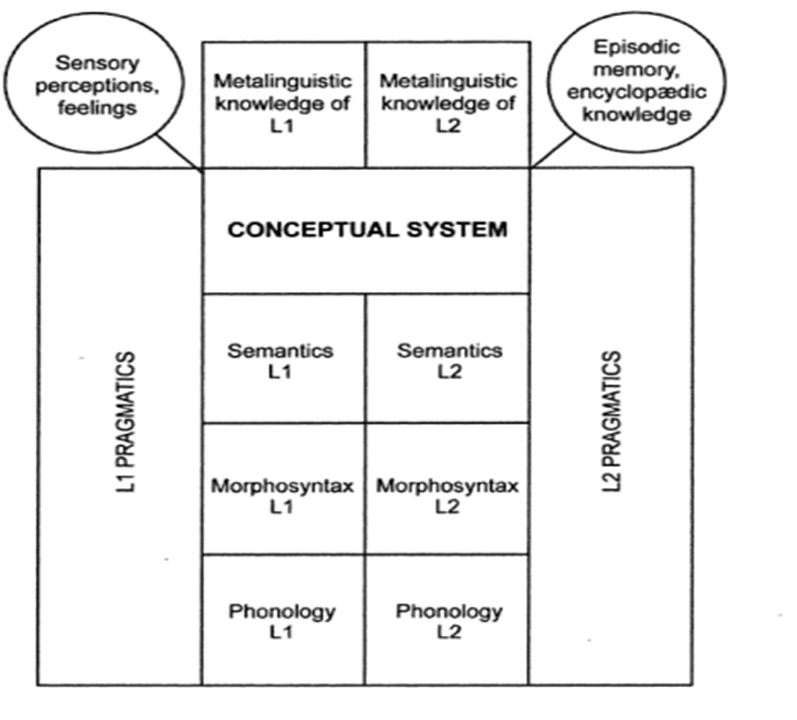
\includegraphics[height=.3\textheight]{figures/Vandevoorde2-img94.png}
\caption{\label{fig:5:91}  Schematic representation of the components of verbal communication (copied from \citealt[227]{paradis_neurolinguistic_2004})}
\end{figure}

The selection of the appropriate conceptual features is driven by lexical meaning \citep[203]{paradis_neurolinguistic_2004}, implying that when a speaker hears a word, the appropriate lexical item is immediately selected. The fact that the speaker is a unilingual or a bilingual does not change anything to the fact that each word is “directly perceived as a word and its meaning” \citep[203]{paradis_neurolinguistic_2004} (the fact that the bilingual perceives that the word is an English or a French word is of no importance to access the lexical item since such knowledge is metalinguistic in nature). This idea is captured as the “Direct Access Hypothesis”, which is also compatible with the previous two hypotheses (the idea of Direct Access can be combined with the idea that the verbal communication system consists of one non-linguistic conceptual level and four independent, but language-dependent subsystems). According to the Direct Access Hypothesis “[l]exical access is language nonselective but sensitive to language-specific characteristics of the input” \citep[205]{paradis_neurolinguistic_2004}. In other words, the lexical item that will be accessed will be the one corresponding to the perceived lexical item in the particular input language, but the language as such does not influence the accessing of the lexical item. This means that bilinguals use the available information (phonological if spoken or orthographic if written) provided by a lexical item to access the item in the according subsystem, not the meta-linguistic knowledge about which language the word pertains to.

Within this hypothesis, translation equivalents are thought to function just as synonyms in a unilingual context (in cross-linguistic priming experiments, translation equivalents are predicted to cause a similar effect as synonyms; \citealp[219]{paradis_neurolinguistic_2004}), and, in general, it is stated that “when a word is activated, its synonym, homophone or translation equivalent should also receive some activation” \citep[219]{paradis_neurolinguistic_2004}. Special attention is given to cognates, which, according to the Direct Access Hypothesis, will be immediately understood “when word forms sufficiently resemble their translation equivalent […]” \citep[218]{paradis_neurolinguistic_2004}. In fact, when a language user knows a word in one language as well as its cognate in another language, both language subsystems will recognize the word “directly in one, and by immediate “completion” in the other” \citep[218]{paradis_neurolinguistic_2004}. In cross-linguistic priming experiments, the fact that no extra processing time is needed is understood as “simultaneous activation of two languages” \citep[219]{paradis_neurolinguistic_2004}. Simultaneous activation (no extra processing time) then reflects “either (1) the similarity of lexical meaning between a word and its translation equivalent at the conceptual level, or (2) the fact that any extra processing time for the recognition of a cognate in the other subsystem is insignificant” \citep[219]{paradis_neurolinguistic_2004}. Consequently, simultaneous activation of two languages will be at its strongest for written cognates, where there is maximal semantic overlap (similarity of lexical meaning) and form overlap (typical for cognates) \citep[219]{paradis_neurolinguistic_2004}.

\subsection{Applying Paradis’ theory to translation}
\label{sec:5.3.2}  
Different from the bilingual speaker’s case, the situation of “simultaneous activation of the two languages” can be assumed to be the normal cognitive state of a translator when he is carrying out a translation task, so that words with identical lexical meaning and their translations will be ``automatically'' activated simultaneously (this would then be the case for close cognates as well as for ``entrenched'' translation equivalent pairs).

The presence of a single conceptual system “does not imply that the same concept corresponds to a lexical item in L\textsubscript{x} and its lexical equivalent L\textsubscript{z} but [implies] that they share some of the same conceptual features, though each may also (and most often does) contain features not included in the other (\citealt{paradis_bilingual_1978, auger_representation_1997,de_groot_lexical_1997,Costaetal2000}; \citealt[198]{paradis_neurolinguistic_2004}). As a consequence, translation equivalents have overlapping, but never identical conceptual representations \citep[12]{kecskes_neurofunctional_2007}. For instance, French \textit{cheveu} [hair growing on human scalps] and \textit{poil} [any other hair] and Dutch \textit{haar} [hair] (example adapted from \citealt[201]{paradis_neurolinguistic_2004}) refer to what Paradis calls the same linguistic concept, but their conceptual representation will differ. The conceptual representation is that part of the linguistic concept which is activated and which consists of “only those relevant features of the linguistic concept […] as restricted by the situation and the linguistic context in which the word is uttered” \citep[12]{kecskes_neurofunctional_2007}. The conceptual representation of French \textit{cheveu} in the sentence \textit{la} \textit{fille} \textit{a} \textit{de} \textit{longs} \textit{cheveux} [the girl has long hair] will be different (other features will be activated) from the conceptual representation of Dutch \textit{haar} in the sentence \textit{de} \textit{hond} \textit{heeft} \textit{lang} \textit{haar} [the dog has long hair] although \textit{haar} and \textit{cheveu} belong to the same linguistic concept. Both \textit{cheveu} and \textit{poil} can be translation equivalents of Dutch \textit{haar}, but \textit{cheveu}, \textit{poil} and \textit{haar} do not share all of their conceptual features, although they have many overlapping features (in fact, Dutch \textit{haar} encompasses the features of both \textit{cheveu} and \textit{poil}). In Paradis’ hypothesis, although the language systems (the subsystems) are independent, conceptual meanings group together conceptual features on the non-linguistic conceptual level. For \textit{cheveu}, \textit{poil} and \textit{haar}, their sets of features will then overlap (\citeyear[13]{kecskes_neurofunctional_2007}) on the non-linguistic conceptual level without being identical. The activation of differential sets of conceptual features works in the same way for unilingual synonyms such as \textit{cheveu} and \textit{poil} as for translation equivalents such as \textit{cheveu} and \textit{haar} or \textit{poil} and \textit{haar} \citep[14]{kecskes_neurofunctional_2007}.

Applied to the case of the bilingual translator who needs to translate Dutch \textit{haar} into French, the following situation arises: the translator, who is constantly primed by the source language, first enters a phase of comprehension. The written form \textit{haar} activates the lexical item \textit{haar} and its meaning on the subsystem level of the Dutch language. A connection is made with the conceptual level, where the lexical item \textit{haar} causes a number of conceptual features to group together according to the specific lexical semantic constraints of \textit{haar} in Dutch as well as according to the pragmatic circumstances evoked by the context \textit{haar} was encountered in. Consider the following \figref{fig:5:92} to be a (simplified) representation of the conceptual features activated by the noun \textit{haar}.

\begin{figure}
% 
\includegraphics[width=\textwidth]{figures/Vandevoorde2-img95.png}
\begin{tabularx}{\textwidth}{|CCCCC|}
\hline
filiform & covers body & covers head & in humans & in animals \\
\LARGE \otimes &\LARGE \otimes &\LARGE \otimes &\LARGE \otimes &\LARGE \otimes \\
\hline
% \bigcirc
\end{tabularx}
\caption{\label{fig:5:92}  Representation of the conceptual features activated by \textit{haar}}
\end{figure}

Depending on the context in which \textit{haar} was encountered, some of the features will be activated, and others not. For the sentence \textit{het} \textit{meisje} \textit{heeft} \textit{lang} \textit{haar} [the girl has long hair], the following conceptual features (\figref{fig:5:93}) will be activated (the fact that the conceptual features `covers head' and `in humans' are simultaneously activated, de-activates the conceptual features ‘covers body’ and ‘in animals’ for \textit{haar} in this sentence):

\begin{figure}
% 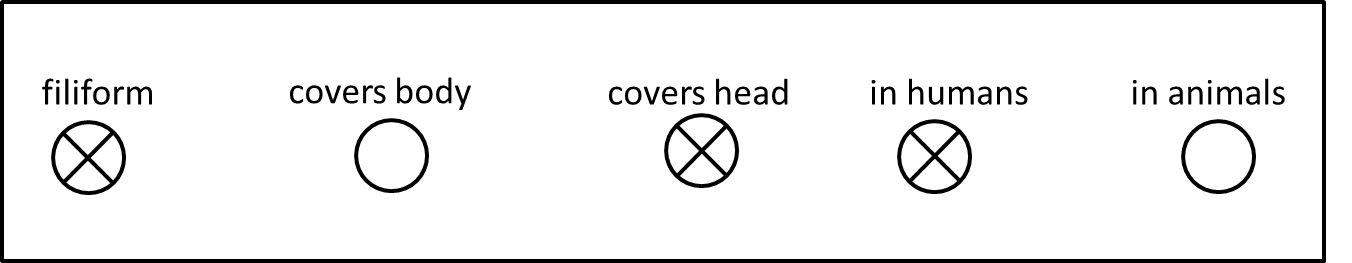
\includegraphics[width=\textwidth]{figures/Vandevoorde2-img96.png}
\begin{tabularx}{\textwidth}{|CCCCC|}
\hline
filiform       & covers body     & covers head   & in humans     & in animals \\
\LARGE \otimes &\LARGE  \bigcirc &\LARGE \otimes &\LARGE \otimes &\LARGE  \bigcirc \\
\hline
\end{tabularx}
\caption{\label{fig:5:93}  Activated conceptual features for \textit{het} \textit{meisje} \textit{heeft} \textit{lang} \textit{haar}}
\end{figure}

For the sentence \textit{de} \textit{hond} \textit{heeft} \textit{lang} \textit{haar} [the dog has long hair], the following conceptual features (\figref{fig:5:94}) will be activated (the activation of ‘covers body’ and ‘in animals’ de-activates ‘in humans’ in this context):

\begin{figure}
% 
\includegraphics[width=\textwidth]{figures/Vandevoorde2-img97.png}
\begin{tabularx}{\textwidth}{|CCCCC|}
\hline
filiform       & covers body     & covers head   & in humans     & in animals \\
\LARGE \otimes &\LARGE  \otimes &\LARGE \otimes &\LARGE \bigcirc &\LARGE  \otimes \\
\hline
\end{tabularx}
\caption{\label{fig:5:94}  Activated conceptual features for \textit{de} \textit{hond} \textit{heeft} \textit{lang} \textit{haar}}
\end{figure}

When the translator now needs to translate these two sentences with \textit{haar} into French, s/he departs from a mental representation already activated by the lexical semantic constraints of the Dutch source language on the basis of which s/he needs to select a realization of this set (or the closest approximation to this set) of conceptual features in the target language (a lexical item in French). For the first sentence, the activated conceptual features `filiform', ‘covers head’ and ‘in humans’ can only lead to the selection of French \textit{cheveu} in the subsystem of the target language (since ‘covers head’ is not activated in \textit{poil}). For the translation of the second sentence, however, the activated conceptual features by \textit{haar} can lead to either \textit{cheveu} or \textit{poil} (the activation of the conceptual feature ‘covers head’ could lead to the selection of \textit{cheveu}, but the activation of ‘covers body’ and ‘in animals’ would lead to \textit{poil}). The conceptual features activated by \textit{cheveu} as well as by \textit{poil} show some overlap (but are not identical) with those activated by \textit{haar}, as the following two Figures 95 and 96 show:

\begin{figure}
% 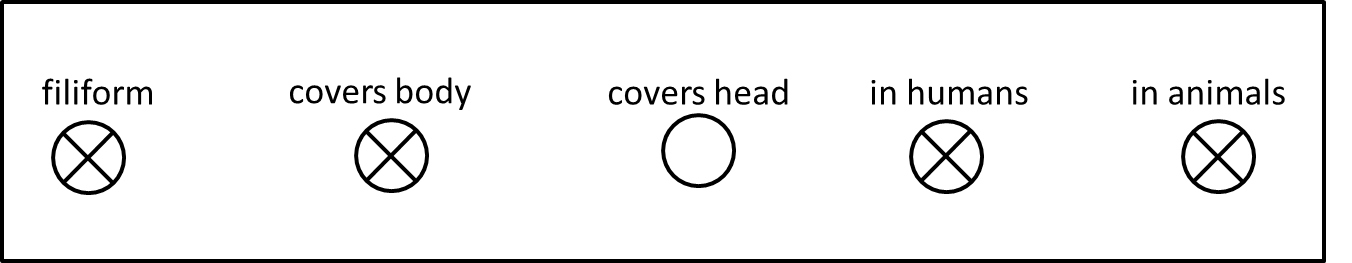
\includegraphics[width=\textwidth]{figures/Vandevoorde2-img98.png}
\begin{tabularx}{\textwidth}{|CCCCC|}
\hline
filiform       & covers body     & covers head   & in humans     & in animals \\
\LARGE \otimes &\LARGE  \otimes &\LARGE \bigcirc &\LARGE \otimes &\LARGE  \otimes \\
\hline
\end{tabularx}
\caption{\label{fig:5:95}  Activated conceptual features for \textit{poil}}
\end{figure}

\begin{figure}
% 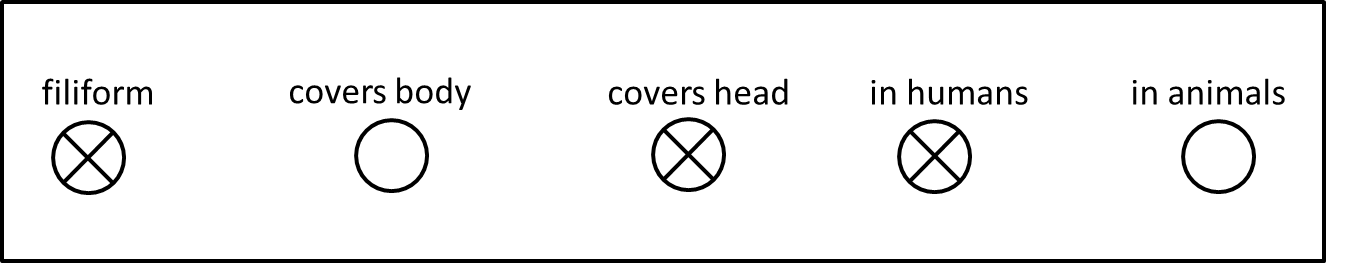
\includegraphics[width=\textwidth]{figures/Vandevoorde2-img99.png}
\begin{tabularx}{\textwidth}{|CCCCC|}
\hline
filiform       & covers body     & covers head   & in humans     & in animals \\
\LARGE \otimes &\LARGE  \bigcirc &\LARGE \otimes &\LARGE \otimes &\LARGE  \bigcirc \\
\hline
\end{tabularx}
\caption{\label{fig:5:96}  Activated conceptual features for \textit{cheveu}}
\end{figure}

When the translator wants to attain sufficient overlap of conceptual features for the second sentence, the constraint on \textit{cheveu} which does not have the conceptual feature ‘in animals’, will prevent the translator from selecting \textit{cheveu} (since the subject of the sentence that needs to be translated refers to an animal). The activation of the conceptual feature ‘in animals’ will then prevail and lead to the selection of \textit{poil}.

Second, when confronted with a sentence such as \textit{de} \textit{actrice} \textit{is} \textit{mooi} [the actress is beautiful], Dutch \textit{actrice} activates the lexical item \textit{actrice} and its meaning in the Dutch language subsystem (just as for \textit{haar}), but, due to the (quasi-)total form and meaning overlap, the French lexical item \textit{actrice} and its meaning are simultaneously activated in the French language subsystem (and a translation is immediately found and can be produced), so that the conceptual system is not used here.

In sum, when a translator carries out a translation task, two scenarios are imaginable. First, the translator’s mind can function from the source language subsystem and arrive, via the common conceptual system, to select a translation in the target language subsystem. This ``strategy'' is called \textit{translating} \textit{via} \textit{the} \textit{conceptual} \textit{system} (\citealt[54--55]{house_towards_2013}; \citeyear{house_translation_2015}; \citeyear[119--20]{house_translation_2016}) (the example of \textit{haar}). When the translator translates via the conceptual system, the bilingual mind first connects the lexical item (verbalized in the source language) to its appropriate concept at the common conceptual level, where the appropriate conceptual features are activated, taking into account the constraints of the source language. Then, crucially, the translator needs somehow to get rid of the constraints which the source language imposes on the concept – s/he needs to consider the nonlinguistic, unconstrained concept – and subsequently select the conceptual features which correspond to the constraints of the target language – in order to be able to select the adequate lexical equivalent in the target language (which shares some of the same conceptual features but not necessarily all features with the source language lexical item). This is where the decoding takes place; and the decision of the translator will eventually generate the production of a translation (or an omission). The translator will thus choose the lexical equivalent which shares a sufficient amount of conceptual features, comply with the constraints of the target language and consider all other constraints that can possibly act upon this choice (cultural, grammatical, pragmatic, etc.). This first ``strategy'' in fact also explains how lack of exact equivalence can be bypassed by the bilingual mind (of the translator).

In the second scenario, due to the considerable form and/or semantic overlap between the source language word and a given target language word (a cognate), the word is activated simultaneously in the source language subsystem as well as its cognate in the target language subsystem. Hence, the translator arrives directly from the source language subsystem to the target language subsystem without processing via the common conceptual system. This second ``strategy'' is called \textit{direct} \textit{transcoding} (\citealt[54--55]{house_towards_2013}, \citeyear{house_translation_2015}, \citeyear[119--120]{house_translation_2016}) (the case of \textit{actrice}).

The importance of form similarity as put forward here is further substantiated by\todo{Ref unclear} \citet[140]{heredia_bilingual_2014}. Although in general bilingual speaker’s contexts “association strengths between L1 and L2 words will be very weak”, they can be strong in the following three cases: for direct translations, for cognates and for so-called “loan-words” (when there is no counterpart in the other language) \citep[141]{heredia_bilingual_2014}. In a translational context with French, English and Dutch, these three cases are certainly not rare, and translators will – in all likelihood – be drawn to the selection of those direct translations, cognates and loan-words in order to translate as “quick and accurately” as possible \citep{kroll_category_1994}.

In addition to the case of cognates, where Paradis hypothesizes direct transcoding, it is very likely that the quick (and accurate) selection of the target language lexical item will take place for lexical items which have a direct translation (cf. also Halverson’s “entrenchment of translation pairs”; \citeyear[15]{de_sutter_developing_2017}). Although this direct translation is not a cognate, the quasi-total overlap of conceptual features and/or the association strength (Halverson’s connectivity) between the source language lexical item and the target language lexical item will favor the fast selection of that particular target-language lexical item. As for loan-words, the translator will become aware that the conceptual features activated by the source language lexical item correspond to extremely few or no conceptual features connected to a verbalization in the target language. Especially when none of the conceptual features are connected to a target language lexical item, the translator can choose to use the exact source language lexical item in the target language. The influence of the strong cross-linguistic associative links of direct translations, cognates and loan-words (and the degree to which these three phenomena exist within a given language pair) can possibly influence the overall translational mechanisms that are applied. In other words, although the translator might ``benefit'' from language similarity (he can process translations ``quicker and more accurately''), form-similarity is likely to have a more prominent influence on the overall semantic representation of translated language when the source language is (lexically) more form-similar to the target language, because the translator seems to rely more on form-similarity (direct transcoding) and less on his conceptual understanding of the meaning of the unit that needs to be translated. Translating via the conceptual system would thus bring translators ``closer'' to the (original) target language semantic representation, though never completely.

\subsection{Applying Paradis’ theory to the resulting semantic representations of inchoativity}
\label{sec:5.3.3}  
Paradis’ framework is now applied to the observations about overall semasiological levelling out in translated language; onomasiological shining through in TransDutch\textsubscript{ENG,} semasiological shining through or normalization for ACTION and STATE AFTER ONSET in translated language and semasiological shining through in TransDutch\textsubscript{FR} for ACTION and SPECIFIC ACTION. I consider our visualizations to be semantic representations of what comes out of the mind – the output of the verbal communication system. The cluster formation in each dendrogram is based on (translational and semantic) overlap and (translational co-occurrence) frequency. Based on the above section, I concluded that direct transcoding can only take place when a number of conditions with respect to semantic and form overlap are fulfilled. As a consequence, it seems plausible that the clustering of lexemes (especially the visualizations such as the ones presented in \sectref{sec:4.6.2} which jointly represent source and target language lexemes) can give indications of direct transcoding or translation via the conceptual system.

The idea of direct transcoding can offer a straightforward explanation for the instances of onomasiological shining through in TransDutch\textsubscript{ENG.}. When the translator is working from English into Dutch, direct transcoding is more likely to take place since cognates between English and Dutch are much more frequent than between French and Dutch. This is confirmed by \citet{schepens_cross-language_2013} who calculated the \textit{relative} \textit{cognate} \textit{frequency} (based on frequency, orthographic and phonetic similarity) for a number of language pairs and found that cognate frequency relative to translation equivalent frequency was much higher for English-Dutch (0.94, meaning that cognates have almost equal frequency of translation equivalents) than for French-Dutch (0.56, meaning that cognates have only little more than half the frequency of translation equivalents; \citealt[4]{schepens_cross-language_2013}). The separate clustering of \textit{opstarten} and \textit{begin} could indicate that direct transcoding is taking place in TransDutch\textsubscript{ENG}. However, the frequency matrix in appendix C shows that \textit{opstarten} and \textit{begin} are also translations of other lexical items, implying that there is also translation via the conceptual system taking place (although the translation of a lexeme by its close cognates does not exclude translation by the conceptual system of course; but for close cognates direct transcoding is more plausible). In contrast to \textit{opstarten} and \textit{begin}, and despite the fact that they also have a close cognate in English, \textit{starten} and \textit{beginnen}, are not forming separate (singleton) clusters. This could indicate that direct transcoding is taking place to a lesser extent for these two items than for \textit{opstarten} and \textit{begin}. No direct transcoding could be hypothesized for TransDutch\textsubscript{FR} since there are simply fewer close cognates between French and Dutch (especially for the field of inchoativity). The translator thus necessarily relies (more prominently) on the strategy of translating via the conceptual system when translating from a language which shares fewer close cognates with the target language such as French, compared to English. This difference could now explain why I did not find instances of onomasiological shining through of translated Dutch from a lexically ``less cognate'' language as French.

Semasiological levelling out in translated language (observed as the inclusion of NON-LEXICALIZED INCHOATIVITY and \textit{eerst} within the reference clusters of both TransDutch fields) can be explained within Paradis’ neurofunctional theory as follows: target language words which do not lexicalize inchoativity or \textit{eerst} have fewer activated conceptual features when used in their inchoative sense than more specific expressions of inchoativity (in these cases, much of the inchoativity is deduced from the context in which these lexemes are used, which implies that these lexemes only activate a minimal amount of conceptual features for inchoativity). When the translator is in search of a target-language lexical item which activates ``enough'' conceptual features so that sufficient overlap with the activated conceptual features of the source language lexical item is established, the selection of a target language lexical item which only activates the minimal sufficient amount of conceptual features is in fact a ``natural choice'' since it constitutes a quick, accurate and ``safe'' solution. This can explain why verbs which do not lexicalize inchoativity become part of the reference cluster (with the effect of semasiological levelling out).

With regard to semasiological shining through or normalization for ACTION and STATE AFTER ONSET in translated language, as well as semasiological shining through in TransDutch\textsubscript{FR} for ACTION and SPECIFIC ACTION, Paradis’ model also offers a possible explanation here (although it must be admitted that my interpretation is speculative and constitutes only one of the many possible ways to interpret these changes in semantic structure). I will take the example of TransDutch\textsubscript{FR} here, where the joint clustering of ACTION and SPECIFIC ACTION as well as the separate clustering of ACTION and STATE AFTER ONSET may be interpreted as semasiological shining through.

When a translator needs to translate \textit{lancer} into Dutch, a number of conceptual features are activated by \textit{lancer} (according to the specific lexical semantic constraints imposed by the verb as well as the context it is used in). The translator needs to select a lexical item in SourceDutch which shows a sufficient amount of overlapping conceptual features with \textit{lancer}. Next, when the translator needs to translate \textit{se} \textit{lancer}, a number of conceptual features will again be activated (just as for \textit{lancer}). The separate clustering of \textit{lancer} (with ACTION) and \textit{se} \textit{lancer} (with STATE AFTER ONSET) in SourceFrench indicates that the activated conceptual features by \textit{lancer} and \textit{se} \textit{lancer} will differ at least in that \textit{lancer} will activate (more) conceptual features relating to ACTION and \textit{se} \textit{lancer} (more) conceptual features relating to STATE AFTER ONSET. The fact that in TransDutch\textsubscript{FR}, ACTION and SPECIFIC ACTION are clustered together, shows that the set of common conceptual features that are maintained when translating \textit{lancer} or \textit{se} \textit{lancer} into Dutch share a (large) amount of the common conceptual features of ACTION and SPECIFIC ACTION, to the point that the conceptual features which usually (in non-translated language) distinguish ACTION from SPECIFIC ACTION are not activated any more, provoking the joint clustering of ACTION and SPECIFIC ACTION in TransDutch\textsubscript{FR}. By the same mechanism, conceptual features of STATE AFTER ONSET (which are activated by \textit{lancer}) will be de-activated because the pragmatic circumstances will impose activation of conceptual features that are common to ACTION and SPECIFIC ACTION but not to STATE AFTER ONSET, provoking simultaneously also the separate clustering of ACTION and STATE AFTER ONSET. The translator’s search for an adequate set of overlapping conceptual features corresponding to a lexical item in the target language subsystem can explain the joint clustering of ACTION and SPECIFIC ACTION as well as the separate clustering of ACTION and STATE AFTER ONSET in translated language.

In sum, the idea of direct transcoding and translation via the conceptual system opens a number of possibilities to explain the differences in semantic structures between translated and non-translated language. However, my interpretation suffers from the same limitations as that of the GPH in that a post-hoc application of such a framework can only go as far as adding an explanatory layer to the observations (it cannot ``test'' the models as such).

\section{Conclusion}
\label{sec:5.4}  
In this chapter, I have made an attempt to explain the main observations of this study on the basis of two cognitively inspired frameworks. I first explored how the GPH could account for the results of this study. I found that the idea of connectivity can explain the observed onomasiological shining through in TransDutch\textsubscript{ENG} as well as semasiological levelling out. Given my post-hoc approach, it appeared however difficult to connect my remaining results to the explanatory framework of the GPH since the revealed differences between the fields of translated and non-translated Dutch were not often connected to salient patterns in neither the source nor the target language.

The second cognitive framework I explored was Paradis’ neurolinguistic theory of bilingualism. Onomasiological shining through could be explained as direct transcoding (which shares the basic idea with connectivity of salient translational relationships). Semasiological levelling out and semasiological shining through could be interpreted within the wider framework as translation via the conceptual system.

The proposed cognitive frameworks have supplied supplementary insights into the structure of the semantic fields and in addition helped to explain where instances of levelling out and shining through on the semantic level might originate. As I already mentioned, a post-hoc application of these frameworks has its obvious limitations. Nevertheless, I hope to have demonstrated the explanatory power of these frameworks, especially when they are combined with methodological instruments such as the visualizations proposed in this study. Much more research is nevertheless needed, so that clear hypotheses about semantic changes in translation can be drawn up a priori and subsequently submitted to these types of frameworks.
